% -*- root: ../thesis.tex -*-
%!TEX root = ../thesis.tex
% ******************************* Thesis Appendix A ****************************
\chapter{Additional works} 
\label{appendix:worshoppapers}
The following work does not fit the storyline of the thesis and is therefore presented here only.
It was extended further due to a lack of time and/or inconclusive results.

\section{Adaptive Inducing Points Selection for Gaussian Processes}

Two important questions raised when using the inducing sparse \ac{GPs} are: how should the inducing points be located and how many points do I need to reach my desired level of accuracy?
This work tries to answer this by creating an adaptive algorithm which also works in an online setting.
A final paper was never written as the parameters regulating the inducing point selection is extremely correlated with the model parameters, and it was complicated to produce a stable algorithm.

\textbf{\underline{Authors:}}\\
Th\'eo Galy-Fajou$^1$, Manfred Opper$^1$\\
\small{$^1$TU Berlin}

\textbf{\underline{Details:}}\\
Type: Workshop article\\
Submitted: June 2020\\
Accepted: July 2020\\
URL: \url{https://drive.google.com/file/d/1IPTUBfY_b2WElTWBIVU4lrbHcXnbTWdB/view}\\
Conference: Workshop Continual Learning (ICML 2020)\\


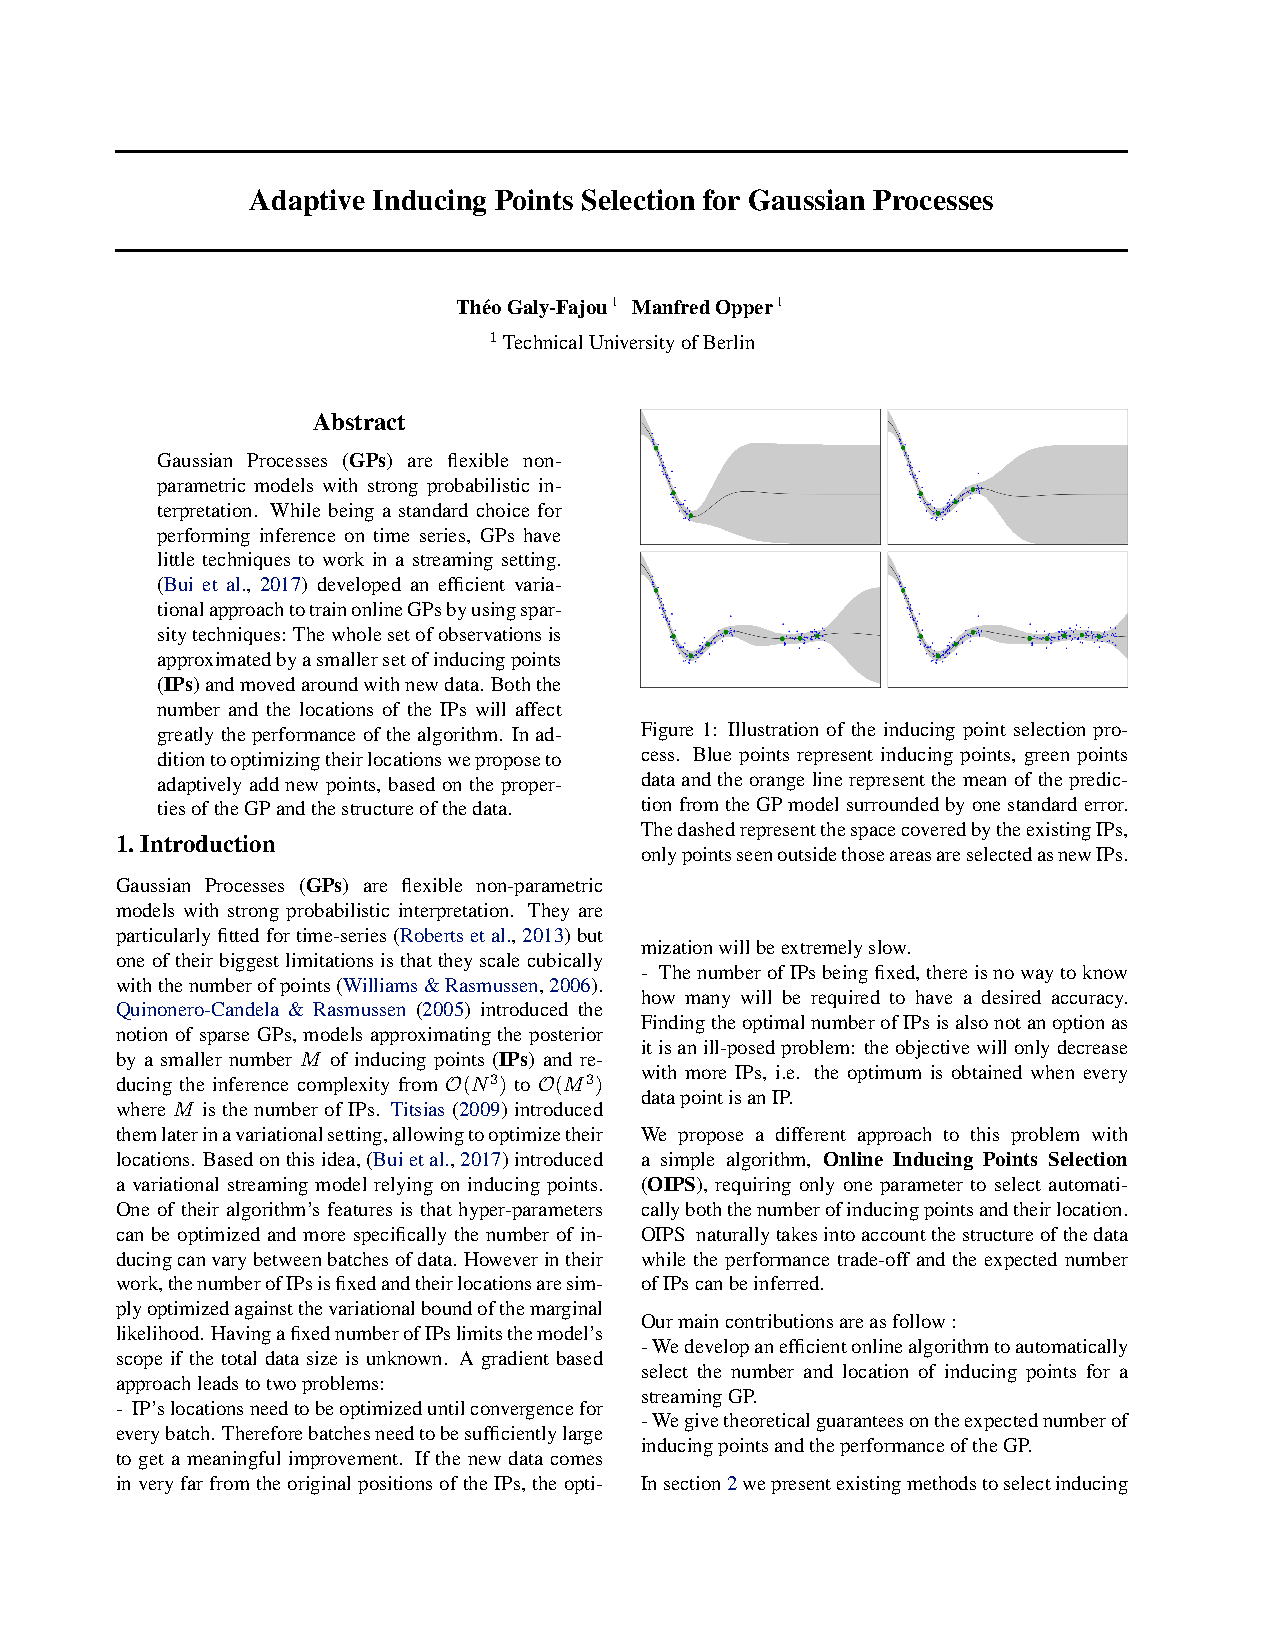
\includepdf[pages=-,pagecommand={},scale=0.95]{./papers/28_CameraReadySubmission_cl_workshop_onlinegp.pdf}

% \section{Evidence Estimation by Kullback-Leibler Integration for Flow-Based Methods}

% \textbf{\underline{Authors:}}\\
% Nikolai Zaki$^1$, Th\'eo Galy-Fajou$^1$, Manfred Opper$^1$\\
% \small{$^1$TU Berlin}

% \textbf{\underline{Details:}}\\
% Type: Workshop article
% Submitted: October 2020\\
% Accepted: December 2020\\
% URL : \url{https://openreview.net/forum?id=LclKtSfmf9I}\\
% Conference: 3rd Symposium on Advances in Approximate Bayesian Inference, 2020\\


% 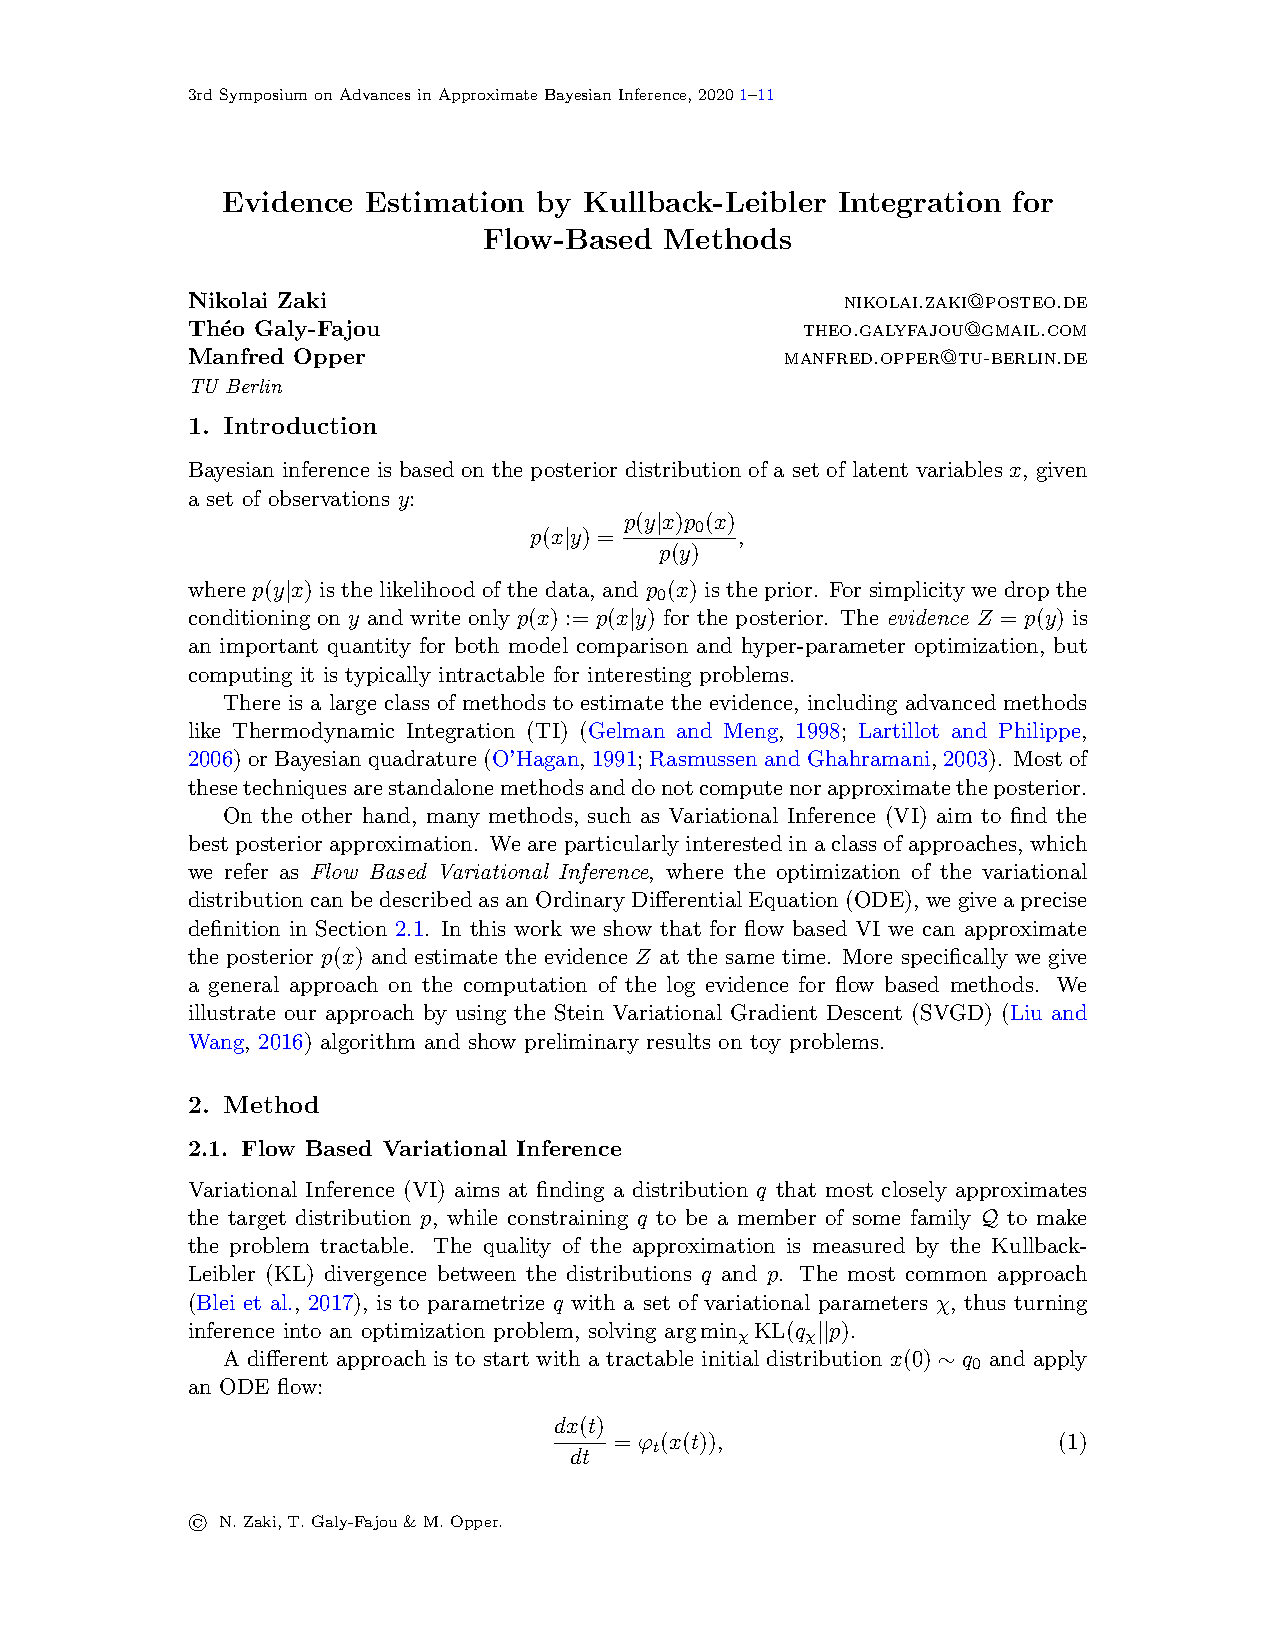
\includepdf[pages=-,pagecommand={},scale=0.95]{./papers/evidence_estimation_by_kullbac.pdf}